\section{Fun Fact}

\begin{frame}{\btitle{pD}}
    \begin{columns}[T,onlytextwidth]
        \begin{column}{0.48\textwidth}
            \centering
            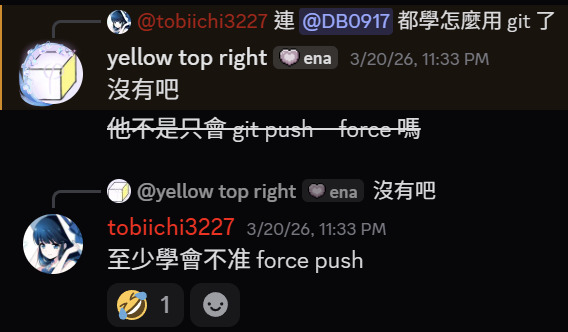
\includegraphics[width=\linewidth,height=0.42\textheight,keepaspectratio]{../pD/statement/db-force-push-1.jpg}

            \small Force push 1 原圖
        \end{column}
        \begin{column}{0.48\textwidth}
            \centering
            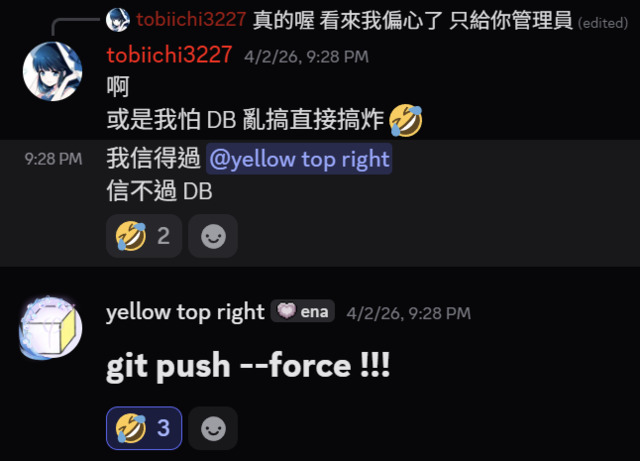
\includegraphics[width=\linewidth,height=0.42\textheight,keepaspectratio]{../pD/statement/db-force-push-2.jpg}

            \small Force push 2 原圖
        \end{column}
    \end{columns}

    \begin{itemize}
        \item 這題其實是我在思考甚麼情況下 Merge 與 Rebase 都會 Conflict，甚麼情況下只有 Rebase 會 Conflict 想出來的
        \item 不要學 DB force push，真的會出事
        \item 我覺得 wonderhoi 一定會來寫這題，沒寫真的要哭了
    \end{itemize}
\end{frame}

\begin{frame}{\btitle{pG}}
    \begin{itemize}
        \item 原本只是隨便想想拿去初賽，結果出完發現太難了倒了
        \item blame 用線代解，直接倒了
        \item 假的 flow 題
    \end{itemize}
\end{frame}